\documentclass[a4paper]{article}

%%%%%%%% CREATE DOCUMENT STRUCTURE %%%%%%%%
%% Language and font encodings
\usepackage[english]{babel}
\usepackage[utf8x]{inputenc}
\usepackage[T1]{fontenc}
%\usepackage{subfig}
\usepackage[table,xcdraw]{xcolor}

%% Sets page size and margins
\usepackage[a4paper,top=3cm,bottom=2cm,left=2cm,right=2cm,marginparwidth=1.75cm]{geometry}

%% Useful packages
\usepackage{enumitem}
\usepackage{amsmath}
\usepackage{amssymb}
\usepackage{graphicx}
\usepackage[colorinlistoftodos]{todonotes}
\usepackage[colorlinks=true, allcolors=blue]{hyperref}
\usepackage{caption}
\usepackage{subcaption}
%\usepackage{sectsty}
%\usepackage{apacite}
\usepackage{float}
\usepackage{titling} 
\usepackage{blindtext}
\usepackage[square,sort,comma,numbers]{natbib}
\usepackage[colorinlistoftodos]{todonotes}
%\usepackage{xcolor}
\usepackage{indentfirst}
\usepackage{amsmath}
\usepackage[linesnumbered,algoruled,boxed,lined]{algorithm2e}
\setlength\parskip{.5\baselineskip plus .1\baselineskip  minus .1\baselineskip}
\setlength{\parindent}{1em}
\definecolor{darkgreen}{rgb}{0.0, 0.4, 0.0}

% \makeatletter
% \def\BState{\State\hskip-\ALG@thistlm}
% \makeatother


%%%%%%%% DOCUMENT %%%%%%%%
\begin{document}



%%%% Title Page
\begin{titlepage}

\newcommand{\HRule}{\rule{\linewidth}{0.5mm}} 							% horizontal line and its thickness
\newenvironment{bottompar}{\par\vspace*{\fill}}{\clearpage}
\center 
\begin{center}
%----------------------------------------------------------------------------------------
%	HEADING SECTIONS
%----------------------------------------------------------------------------------------

\includegraphics[scale=0.8]{upclogo.png}\\[2cm] % Include a department/university logo - this will require the graphicx package
 
%\textsc{\LARGE Polytechnical University of Catalonia}\\[1cm] % Name of your university/college
\textsc{\Large Master in Innovation and Research in Informatics}\\[0.5cm] % Major heading such as course name
\textsc{\large Advanced Human Languages Technologies}\\[5cm] % Minor heading such as course title

%----------------------------------------------------------------------------------------
%	TITLE SECTION
%----------------------------------------------------------------------------------------

\HRule \\[0.4cm]
{ \huge \bfseries Recognition and Interactions of Drugs}\\[0.4cm] % Title of your document
\HRule \\[1.5cm]
 
%----------------------------------------------------------------------------------------
%	AUTHOR SECTION
%----------------------------------------------------------------------------------------
\begin{bottompar}
\begin{minipage}{0.5\textwidth}
\begin{flushleft} \large
\emph{Authors:}\\
Asaf Badouh \\ Pau Rodríguez Esmerats % Your name
\end{flushleft}
\end{minipage}
~
\begin{minipage}{0.4\textwidth}
\begin{flushright} \large
\emph{Professors:} \\
Lluís Padró Cirera \\ Horacio Rodríguez Hontoria   % Supervisor's Name
\end{flushright}
\end{minipage}\\[2cm]

% If you don't want a supervisor, uncomment the two lines below and remove the section above
%\Large \emph{Author:}\\
%John \textsc{Smith}\\[3cm] % Your name

%----------------------------------------------------------------------------------------
%	DATE SECTION
%----------------------------------------------------------------------------------------

{\large \today}\\[2cm] % Date, change the \today to a set date if you want to be precise
\end{bottompar}
\end{center}
\end{titlepage}

\setcounter{tocdepth}{2}
\tableofcontents
\pagebreak

% \begin{abstract}


% \end{abstract}

\pagebreak

\section{Introduction}


Drug name recognition (DNR) is a critical step for drug information extraction.
DNR is the first step to identifying unknown drug interactions (DDI).
DDI is broadly described as a change in the effects of one drug by the presence of another drug.
Because of the lack of labeled corpora, early studies on DNR are mainly based on ontologies and dictionaries.
To promote the research on drug information extraction, MAVIR research network and University Carlos III of Madrid in Spain organized two challenges successively: \textbf{DDIExtraction 2011} and \textbf{DDIExtraction 2013}. 
Both of the two challenges provide labeled corpora that can be used for machine learning-based DNR.\\
We are presenting several approaches to solve \textbf{SemEval-2013 Task 9.1 and Task 9.2}. 


\section{General Approach}

    
   Out of the two tasks of the competition, we implemented two different models (SVM and CRF) for the Drug Name Recognition task (task 9.1) and one model (SVM) for the Drug-Drug Interaction task (task 9.2). This section introduces the general approach followed for each of the models implemented. A general schema is shown in figure \ref{architecture}. The different ideas for features and model configuration have been extracted from different papers $\cite{liu_tang_chen_wang_fan_2015,kim_liu_yeganova_wilbur_2015,ratinov_roth_2009,liu_tang_chen_wang_2015}$.\\
   
\begin{figure}[H]
\centering
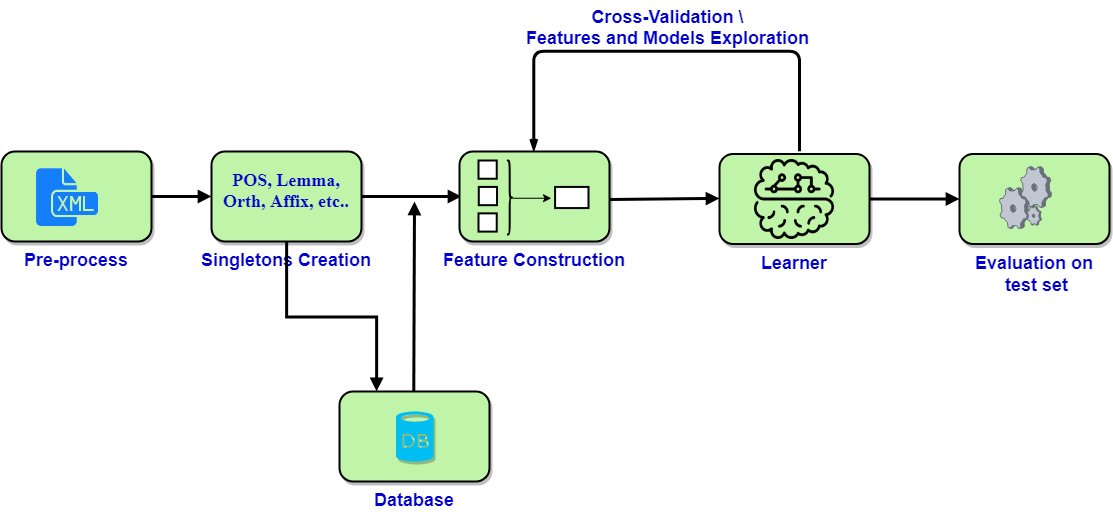
\includegraphics[scale=0.3]{ProcessCV.png}\caption{architecture}\label{architecture}
\end{figure}

   Our implementation, based on Python 3, starts with the parsing of the xml files that contain training and test samples of medical texts with two or more drugs mentioned in it. This first component basically traverses the folder that contains a set of xml files and creates a Python dictionary out of the information in it.\\
   The next software component, is in charge of extracting all the features that our learner model will use to train or to predict. This includes the most basic ones, already present in the xml file, like the word or sentence, or derived features like the BIO tag, the type of interaction for each drug pair , the POS-tag, lemma and orthographic features, all extracted using Freeling from the Python API. Finally, for more complex features, like Word2vec coordinates, dictionary lookup or dependency tree trigram frequencies, this component will write intermediate and final results to a file on disk.\\
   The next module in the chain will be in charge of selecting from the generated features (from memory or disk), the final feature vector that will be feed to the model for training or prediction  according to a configuration file that orchestrated the whole process.\\
   Finally, a learning model will be created and will use the features from the training data set to be trained and the features from the test data set to perform the predictions and evaluate its performance. We used scikit-learn and sklearn-crfsuite for the implementation of the learners.\\
   Due to our constrained time and resources, we performed feature selection and model selection by exploring different configurations of features and models in the two training and testing datasets. Our preferred approach would have been to preform model selection using crossvalidation before evaluating the selected model in the test set. Feature selection could also be done based on an analysis of the data and features, like frequency of appearance of each feature or entropy analysis.\\
   
   The models are trained from the training set of both Drugbank and Medline all mixed, but tested on each test set separately, in order to be able to use the official evaluation java code for the task 9.1 and 9.2 of SemEval'13. \\
   
The different experiments include exploring the results of training the svm model with different sets of features and window sizes, as well as with different model parameters. All the experiments are orchestrated by configuration files using the YAML format, where keys and values define the training and test set, the type of model, the features and window size as well as saving the results of the evaluation of the model.

  Further sections will explain the specific implementation for each trainer model and task.
    


\section{Models}


\subsection{DNR with SVM}

The first implementation trains a Support Vector Machine model to perform classification of BIO tag for each word as a means of Drug Name Recognition. All code is based on Python 3 and Scikit-learn and uses modules for interacting with Freeling, perform the lookup of words on a DrugBank lookup and the like. The model used is a linear support vector machine, which will use the DictVectorizer library from Scikit-learn to transform the feature vector into a suitable format consisting of only binary variables. 

\textbf{Features}

The complete set of features prepared for this model are the following:
\begin{table}[H]
\centering
\begin{tabular}{lcl}
\multicolumn{3}{l}{DNR features}                                                                                                               \\ \hline
$f_{1}$ & Word feature             &                                                                                                                               \\
\rowcolor[HTML]{DAE8FC} 
$f_{2}$ & Part-Of-Speech           &                                                                                                                               \\
$f_{3}$ & Lemmatization           &                                                                                                                               \\
\rowcolor[HTML]{DAE8FC} 
$f_{4}$ & Orthographic - basic features     & \begin{tabular}[c]{@{}l@{}}5 classes: \\ all-capitalized, is-titlecase,all-digits,\\ alphanumeric, hyphen or not\end{tabular} \\
$f_{5}$ & Orthographic - affix features           & Prefixes and suffixes of the length 3,4,5                                                                                     \\
\rowcolor[HTML]{DAE8FC} 
$f_{6}$ & Orthographic - Word shape features      & \begin{tabular}[c]{@{}l@{}}Generalized word class: Xxxxx00xxOxx \\ Brief word class: Xx0xOx\end{tabular}                      \\

$f_{7}$ & Dictionary features      & Lookup on Drugbank                                                                                            \\
\rowcolor[HTML]{DAE8FC} 
$f_{8}$ & Chunk feature            &    NLTK noun phrase chunking tag                                                                                                                         \\
$f_{9}$ & Word Embeddings features & Word2Vec and classification                                                                                                  
\end{tabular}
\caption{DNR features}
\label{table:DNRfeatures}
\end{table}
The drug name lookup is performed on the Drugbank dictionary xml file, parsed in memory as a Python dictionary that allows to query for existence of the word as a key. The chunker feature is obtained from NLTK named entity chunker, returning chunk and chunkGroup for each word in the sentence. 
The Word2Vec feature was obtained from a pretrained 200 window length Word2Vec model from PubMed, where the coordinates of each word where added to the feature vector.
The BIO tag class type is obtained by processing the indications of char offsets for entities in each sentence. In order to avoid any conflict with the Freeling analyzers, the BIO tag matching is done after tokenization and pos taging modules of Freeling are executed. All the orthographic are obtained from the words and their basic lemma and POS-tag features in an adjustable window from 0 to 5. 

\textbf{Feature vector}

The SVM model is trained on a word features basis. This includes all the possible features of a word and the words in a context window of 0 to 5.  This means that the model to be trained will receive a feature matrix consisting of a feature vector for each word of each sentence in the training data set. The structure of the feature vector for each word is shown in the figure \ref{dnrsvm}.

\begin{figure}[H]
\centering
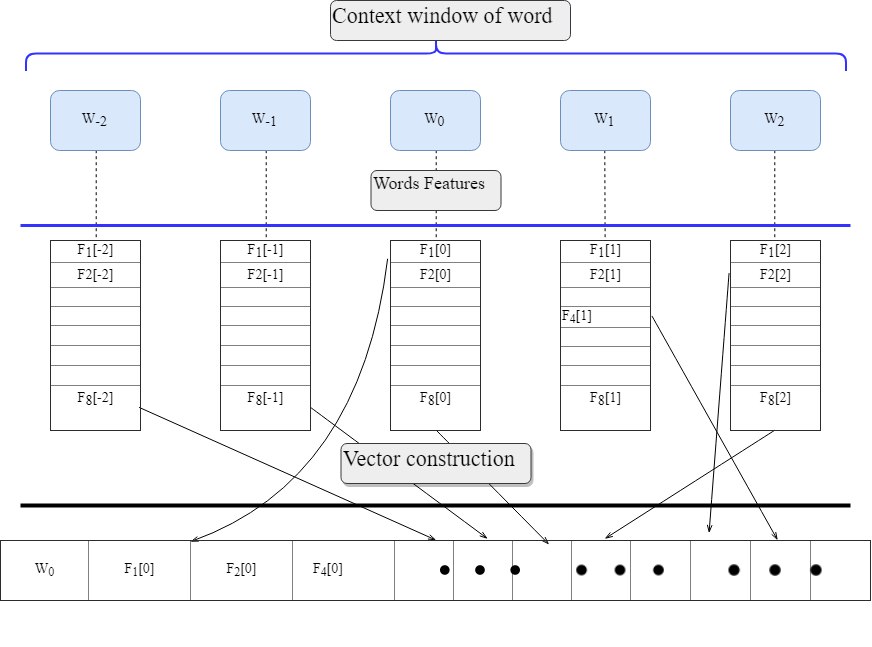
\includegraphics[scale=0.3]{VectorConstruction.png}\caption{DNR-SVM feature vector}\label{dnrsvm}
\end{figure}







\subsection{DNR with CRF}

The second implementation trains a Conditional Random Fields model to perform classification of BIO tag for each word as a means of Drug Name Recognition. All code is based on Python 3 and Scikit-learn and sklearn-crfsuite. As before it uses modules for interacting with Freeling, perform the lookup of words on a DrugBank lookup and the like. This time, the model feature matrix input will be the sequence of features for each word of a sentence. 

\textbf{Features}

The complete set of features prepared for this model is the same used in the previous smv model \ref{table:DNRfeatures}.

\textbf{Feature vector}

The CRF model is trained on a sequence of word features basis. This includes all the possible features of a word and the words in a context window of 0 to 5, concatenated in a sequence for each sentence in the training data set. The structure of the feature vector for each word is shown in the figure \ref{dnrcrf}.


\begin{figure}[H]
\minipage{0.5\textwidth}%
  \centering
  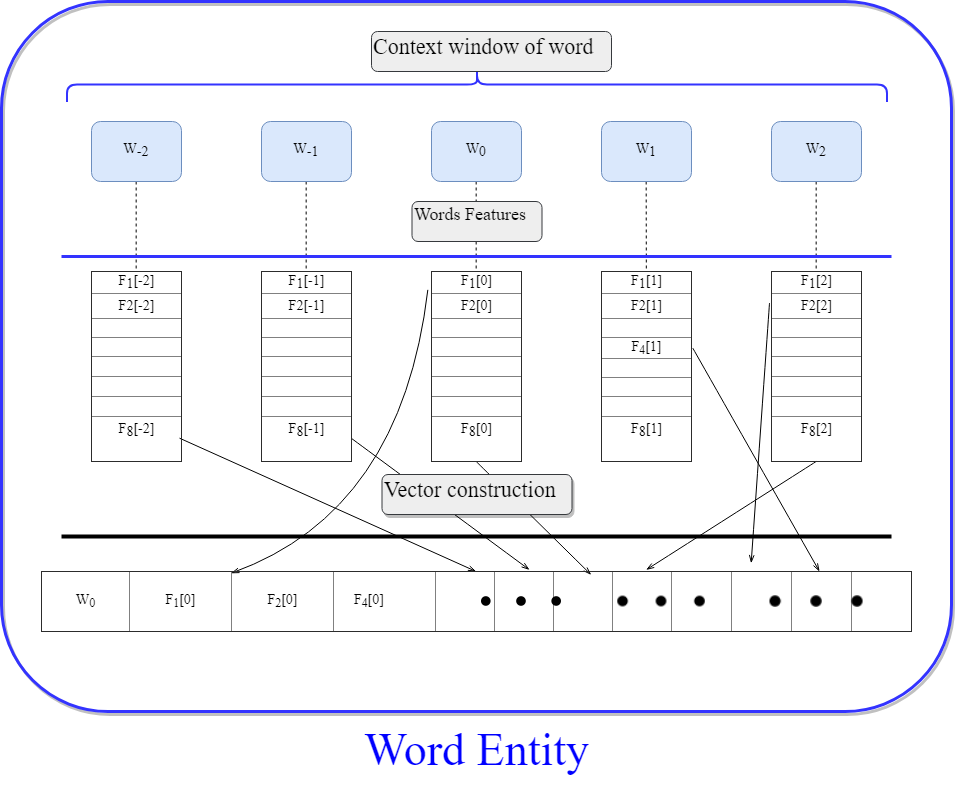
\includegraphics[width=0.8\linewidth]{wordEntity.png}
  \caption{Encapsulation of word features}\label{groupwordfeatures}
\endminipage\hfill
\minipage{0.5\textwidth}
    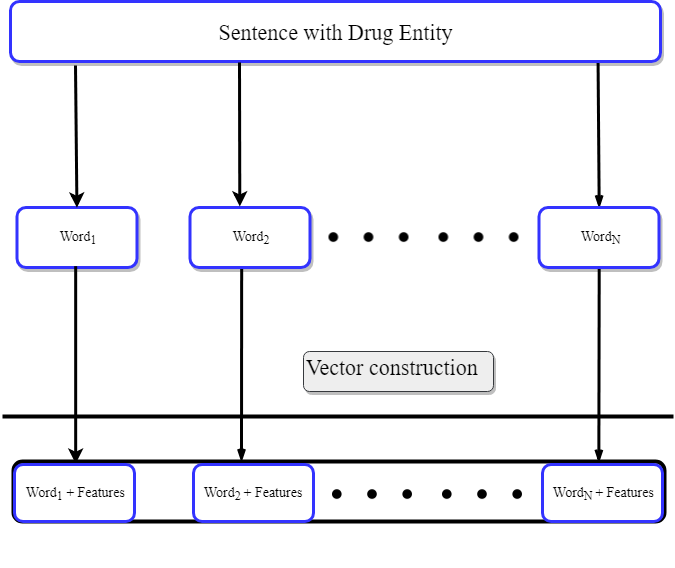
\includegraphics[scale=0.3]{CRF.png}\caption{DNR-CRF feature vector}\label{dnrcrf}
\endminipage
\end{figure}











\subsection{DDI with SVM}

The third implementation trains a Support Vector Machine model to perform Drug-Drug interaction detection and classification for each drug pair appearing in each sentence. All code is based on Python 3 and Scikit-learn. As before it uses modules for interacting with Freeling, perform the lookup of words on a DrugBank lookup and the like. This time, the model feature matrix input will contain features from words in the sentence, and features extracted from the sentence.

\textbf{Features}

%The complete set of features prepared for this model is the same used in the previous smv model (this time only applied to each drug of the pair), but adding features from the context of the sentence.

For the second task to detect drug drug interactions, we have used the single word features for each entity word  \ref{table:DNRfeatures} (in the pair) also with a context window of 3. Then we have added the features derived from the dependency tree (appearances of frequent trigrams, words, lemma, pos. We also added counts of specific POS tags (verbs , determiners, etc).

\begin{table}[H]
\centering
\begin{tabular}{lll}
\multicolumn{3}{l}{Drug-Drug Interaction Features}                                       \\ \hline

$f_{1}$ & All DNR SVM features        & for each entity of the pair   \\
\rowcolor[HTML]{DAE8FC} 
$f_{2}$ & All DNR SVM features in a window        & \begin{tabular}[c]{@{}l@{}}for each word  \\ in a window 0 to 5 \end{tabular}                      \\
$f_{3}$ & Appearance of most frequent 3-gram sequences & from dependency tree shortest path    \\
\rowcolor[HTML]{DAE8FC} 
$f_{4}$ &  Appearance of most frequent Word/Lemma  &        \\
$f_{5}$  & Appearance of most frequent POS  & from CFG parse tree shortest path    \\
\rowcolor[HTML]{DAE8FC} 
$f_{6}$ &  Word count in the shortest path  & from dependency tree shortest path        \\
$f_{7}$ &  Counts of POS tags in sentence   &  specific tags: VB, CC, MD, DT

\end{tabular}
\caption{DDI features}
\label{table:DDIfeatures}
\end{table}




For the Word embedding feature, we used pre-processed database from Pubmed$^{\cite{PubMedDatabase}}$, that contains a Word2Vec model with a 200 words context size. We were'nt able to use this feature due to memory limitation (200 float values per word).\\
For the contextual features, used in the drug drug interaction task, we created different parse trees (Dependency and CFG). In figure \ref{fig:deptree}  we have an example of a dependency tree in a sentence with 2 drugs . We extract the shortest path from the parse tree for each pair interaction and sentence. Then for each shortest path we extract the trigrams, words, lemma , pos and we count how many times each of them appears in the whole training data set. Finally we keep the more frequent ones with a specific threshold (50 for memory size reasons). And finally the feature for each pair- sentence will be the binary var that indicates each of the frequent words/trigrams/etc is in the sentence's shortest path or not.

\textbf{Feature vector}

The SVM model for DDI is trained on a sentence feature vector basis. This includes all the possible features of each drug word in a pair and the words in a context window of 0 to 5, plus the sentence features which are appearances of frequent trigrams, words, lemmas and postags from the dependency tree, as well as counts of POS tags and words. The structure of the feature vector for each word is shown in the figure \ref{fig:ddisvm}.




\begin{figure}[H]
\minipage{0.5\textwidth}%
  \centering
  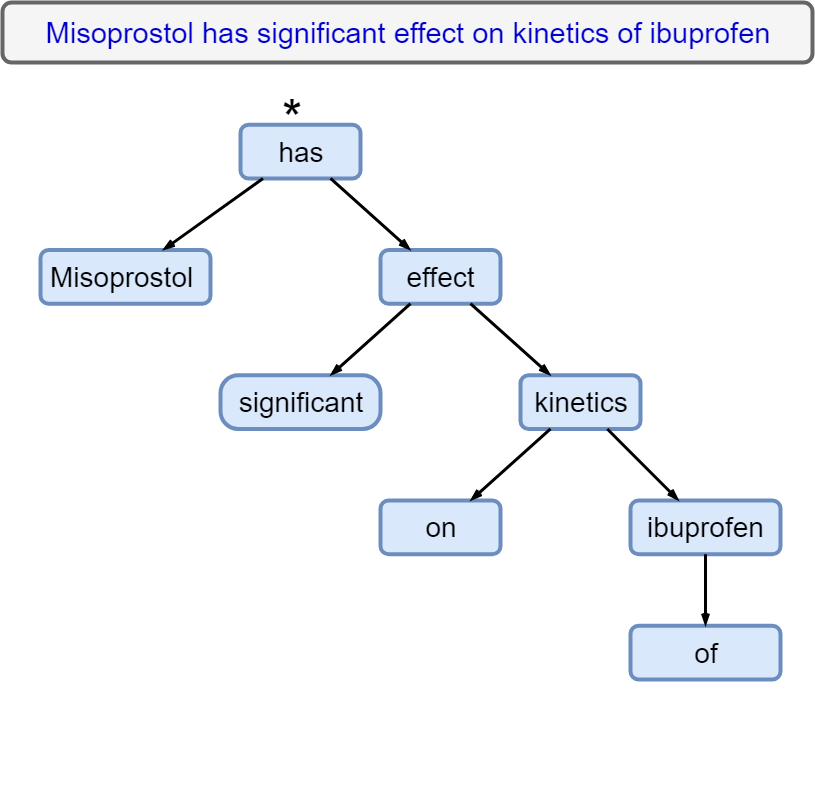
\includegraphics[scale=0.25]{tree.png}
  \caption{Dependency tree }\label{fig:deptree}
\endminipage\hfill
\minipage{0.5\textwidth}
    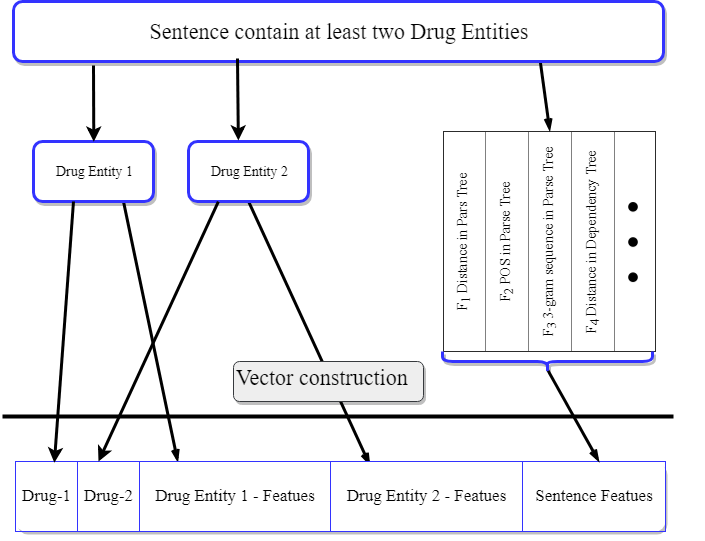
\includegraphics[width=\linewidth]{DDI.png}
  \caption{Feature vector for DDI task}\label{fig:ddisvm}
\endminipage
\end{figure}














\section{Experiments}

The following table summarizes the results of the experiments performed. In blue we highlighted our best models for each task, and in read there is the corresponding best models of the SemEval 2013 competition for each task respectively.

\begin{table}[H]
\centering
\scalebox{0.7}{
\begin{tabular}{ |l|c|c|c|c|c|c|c|c|c|c|c|} 
 \hline
 	Name & Type & Algo. & Features & \# Ftrs & Window & Prec & Rec & F1 & M-Prec & M-Rec & M-F1\\
 \hline
 \rowcolor[HTML]{DAE8FC}
 		\small{ d24tMDmNERaCRFw1m10 } & NER & CRF & pos,ort+pos,ort  &  57 &  -1:+1  &  0.9 & 0.85 & 0.87  &  0.92 & 0.65 & \textbf{0.71} \\
 		\small{ d22btDBmNERaCRFw3m5 } & NER & CRF & pos,ort,lo+pos,ort  &  21 &  -3:+3  &  0.9 & 0.82 & 0.86  &  0.92 & 0.63 & 0.7 \\
 		\small{ d23tDBmNERaLSVMw3m0 } & NER & SVM &
 		
 		\begin{tabular}{c} 
   
 		    lm,pos,lo,chg,ort \\
        
 			+ pos,lo,chg,ort \\ 
 		 \end{tabular}
 			
 			  &  21 &  -2:+2  &  0.83 & 0.79 & 0.81  &  0.64 & 0.54 & 0.58 \\
 		
 		% DrugBank Winner for macro-F1
 		
 		%WBI	3	

 %\hline
 \rowcolor[HTML]{FFCCC9}
 		\small{ SemEval'13	WBI(DrugBank) } & NER &  &   &   &    & 0.921 & 0.914  & 0.917  &  0.653 & 0.659 & \textbf{0.656} \\
\rowcolor[HTML]{FFCCC9}
 		\small{ SemEval'13	UTurku(MedLine) } & NER &  &   &   &    & 0.809 & 	0.521 & 0.634 &  0.649	& 0.528 & \textbf{0.582} \\
 		%remoark our model is overfitted!
 \hline
 
  \rowcolor[HTML]{DAE8FC}
 \small{ ddi006m65(DrugBank) } & DDI & SVM & ort+ort  & 80 &  -3:+3  &  0.6513 & 0.448 & 0.5308  &  0.5778 & 0.3415 & \textbf{0.4293} \\
 		
\small{ ddi006m53(DrugBank) } & DDI & SVM & lm,ort+lm,ort &  96 &  -3:+3  &  0.5748 & 0.4695 & 0.5168  &  0.4292 & 0.3024 & 0.3548 \\

\small{ ddi007m22(MedLine) } & DDI & SVM & 

\begin{tabular}{c} 
   
 		    pos,ort+sent \\
        
 			+ tw,tri,tl,tp \\ 
 		 \end{tabular}
 

                                &  113 &  -3:+3  &  03492 & 02316 & 0.2785  &  05099 & 02531 & 0.3383 \\

 
	
	
 \rowcolor[HTML]{FFCCC9}
\small{ SemEval'13	FBK-irst(DrugBank) } & DDI &  &   &  & &  0.816	& 0.838	& 0.827   &  0.708 &	0.639 &	\textbf{0.672} \\
 \rowcolor[HTML]{FFCCC9}
\small{ SemEval'13	FBK-irst(MedLine) } & DDI &  &   &  & & 0.558 &	0.505 &	0.53  &  0.384 &	0.514 & \textbf{0.44} \\
 		
 		


\hline
 
\end{tabular}
} %scale
\end{table}




\section{Conclusions}
We observe that our CRF model for DNR has a similar performance than the winner of the 2013 SemEval task. In fact, we should perform crossvalidation with our best 3 models, and evaluate the one that generalizes better over validation data. Otherwise we can say that we are overfitting over the testing data set, and we cannot assure that the model will generalize well.\\
We also observe that our model for DDI task obatins a similar performance than the second best model of the SemEval 2013 task 9.2. However, all the models that we have trained for this DDI task have been performing around 35\% of the Macro F1 score and this particular case obtains 42\% by limiting the training data to 1000 pairs of drug interactions. We conclude that due to classe imbalance, the limitation over the training set has somehow balanced the classes allowing the model to perform better. Again, with this treatment we cannot assure that the model will generalize as expected.


We proposed a series of improvements over the current work:
\begin{itemize}
    \item Word embedding - use a more suitable ready-made word2vec db (with less dimensions) or perform a K-means clustering to cluster words based on their word2vec vectors. It has been proposed as a third alternative solution to use the word2vec model to obtain the mosst similar word from the word2vec model for an input word. This resulting similar word could be searched in the lookup over the Drugbank dictionary to see if it is a drug name or not. All those approaches will have to be done by preprocessing the training and test set and saving the intermediate results on files on the disk.

    \item feature selection by frequency of appearance in the dataset, or entropy computation
    \item model selection by cross-validation

\end{itemize}



\newpage
\nocite{*}
\bibliographystyle{unsrt}
\bibliography{references}
\end{document}